\documentclass[a4paper,12pt]{article}

% Pakete einbinden
\usepackage[utf8]{inputenc}
\usepackage[T1]{fontenc}
\usepackage{hyperref}
\usepackage{makeidx}
\usepackage{xcolor}
\usepackage{amsmath}
\usepackage{listings}
\usepackage{qrcode}
\usepackage{tikz}
\usepackage{graphicx}
\graphicspath{ {./images/} }

\makeindex

% Dokumentbeginn
\begin{document}

% Titelseite
\title{Experimente Mit Alu- Kohlenstoffbatterien}
\author{Alexander Borca, Andrey Kalyanov und Yaron Traub}
\date{\today}
\maketitle

% Abstract
\begin{abstract}
\noindent Dieses Dokument demonstriert die Nutzung von LATEX mit Features wie Schriftformatierungen, mathematischen Formeln, Verweisen, QR-Codes, Grafiken, Tabellen und mehr.
\end{abstract}

% Inhaltsverzeichnis
\tableofcontents
\newpage

% Liste der Abbildungen
\listoffigures
\newpage

% Hauptteil (Beispielinhalt)
\section{Einleitung}
In den beiden Experimenten wurden unterschiedliche Methoden zur Herstellung von Batterien mit Kohlenstoff und Papier untersucht.

\section{Versuch mit Bleistift-Schicht und Batterie}

Wir trugen mehrere Schichten auf Papier auf, indem wir zwei unterschiedlich feste Bleistifte verwendeten.

\begin{figure}[h!]
\centering
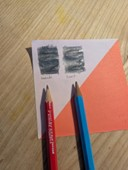
\includegraphics[width=0.5\textwidth]{Bild1} % Ersetze 'Bild1' mit dem tatsächlichen Dateinamen
\caption{Auftragen der Schichten mit verschiedenen Bleistiften}
\label{fig:bild1}
\end{figure}

Mit einem Multimeter überprüften wir, wie gut die aufgetragene Schicht leitete und ob sie überhaupt leitfähig war. Der weichere Bleistift ermöglichte es, mehr Schichten aufzutragen, ohne dass das Papier riss, weshalb diese Schicht besser leitete.

\begin{figure}[h!]
\centering
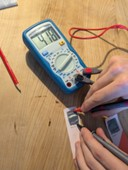
\includegraphics[width=0.5\textwidth]{Bild2} % Ersetze 'Bild2' mit dem tatsächlichen Dateinamen
\caption{Messung der Leitfähigkeit mit einem Multimeter}
\label{fig:bild2}
\end{figure}

Anschließend befestigten wir je einen Draht mit Klebestreifen am Papier und verbanden ihn mit der Kohlenstoffschicht, indem wir leitende Farbe verwendeten.

\begin{figure}[h!]
\centering
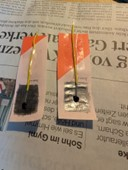
\includegraphics[width=0.5\textwidth]{Bild3} % Ersetze 'Bild3' mit dem tatsächlichen Dateinamen
\caption{Befestigung der Drähte mit Klebestreifen}
\label{fig:bild3}
\end{figure}

Danach klebten wir ein Stück Aluminiumprofil, das wir zuvor auf den größeren Flächen leicht abgeschliffen hatten, auf das Papier und verbanden es mit einem Kabel.

\begin{figure}[h!]
\centering
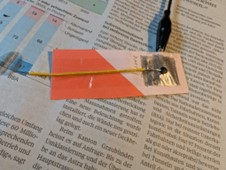
\includegraphics[width=0.5\textwidth]{Bild4}
\caption{Befestigung des Aluminiumprofils}
\label{fig:bild4}
\end{figure}

Als Elektrolyt für unsere Batterie nutzten wir eine Kochsalzlösung, in die wir die Batterie eintauchten, wobei wir darauf achteten, dass jeweils nur ein Kabel im Wasser war. Wie im Bild zu sehen ist, konnte die Batterie tatsächlich Spannung erzeugen.

\begin{figure}[h!]
\centering
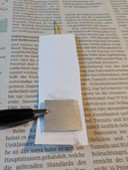
\includegraphics[width=0.5\textwidth]{Bild5}
\caption{Test der Batterie in Kochsalzlösung}
\label{fig:bild5}
\end{figure}

Dies hielt jedoch nicht lange an, da die Farbe wasserlöslich ist und sich das Papier wölbte, wodurch der Kontakt zum Aluminiumprofil beeinträchtigt wurde.

\begin{figure}[h!]
\centering
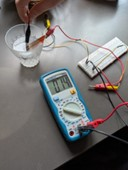
\includegraphics[width=0.5\textwidth]{Bild6}
\caption{Probleme mit der Leitfähigkeit aufgrund der Papierwölbung}
\label{fig:bild6}
\end{figure}



\section{Schriftformatierungen}
\textbf{Fettdruck}, \textit{Kursivdruck}, \textcolor{blue}{blaue Schriftfarbe}, \Large manuell angepasste Schriftgrösse.

\section{Mathematische Formeln}
Unnummerierte Formel:
\[
a^2 + b^2 = c^2
\]
Nummerierte Formel:
\begin{equation}
\int_{0}^{\infty} e^{-x^2} dx = \frac{\sqrt{\pi}}{2}
\label{eq:gauss}
\end{equation}

Verweis auf die nummerierte Formel \eqref{eq:gauss} im Text.

\section{Verweise}
Dieser Abschnitt enthält einen Verweis auf \hyperref[sec:tabellen]{Abschnitt \ref*{sec:tabellen}} auf Seite \pageref{sec:tabellen}.

\section{Externe Links}
Ein Link zu \href{https://www.latex-project.org}{LATEX-Projektseite}.

\section{QR-Code}
Ein QR-Code zur LATEX-Projektseite:
\qrcode{https://www.latex-project.org}

\section{Selbsterstellte Grafiken}
Eine einfache Grafik:
\begin{tikzpicture}
\draw[thick,->] (0,0) -- (2,0) node[right]{x};
\draw[thick,->] (0,0) -- (0,2) node[above]{y};
\draw[thick] (0,0) -- (1,1);
\end{tikzpicture}

\section{Bilder}
Ein eingebundenes Bild:
\begin{figure}[h!]
\centering
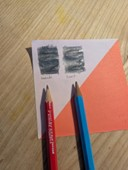
\includegraphics{Bild1}
\caption{Eine Beispielabbildung}
\label{fig:beispiel}
\end{figure}

\section{Codelisting}
Ein Beispielcode:
\begin{lstlisting}[language=Python, caption={Beispielcode in Python}]
def hello_world():
    print("Hello, world!")
\end{lstlisting}

\section{Tabellen}
\label{sec:tabellen}
Eine Beispielstabelle:
\begin{table}[h!]
\centering
\begin{tabular}{|c|c|c|}
\hline
A & B & C \\
\hline
1 & 2 & 3 \\
\hline
4 & 5 & 6 \\
\hline
\end{tabular}
\caption{Eine einfache Tabelle}
\end{table}

\section{Fussnoten}
Ein Beispiel für eine Fussnote\footnote{Dies ist eine Fussnote.} im Text.

% Bibliographie
\newpage
\bibliographystyle{plain}
\bibliography{literatur}

% Index
\newpage
\printindex

\end{document}
